\chapter{Related Work}
\label{chap:related-work}
\thispagestyle{fancy}

\section{\acrlong{utaut}} \label{sec:utaut}

\textcite{Venkatesh2016UnifiedTO} synthesized several models related to technology acceptance and the theory of planned behavior into the \acrfull{utaut}. The \acrshort{utaut} aims to explain the degree of acceptance of the use of information technology and assesses whether a user will be able to accept a new technology.

The \acrshort{utaut} is built upon four key factors: performance expectancy, effort expectancy, social influence and facilitating conditions. The first three factors have a direct impact on the intention to use (behavioral intention) the technology. Moreover, the intention to use is also indirectly influenced by four moderators: gender, age, experience and voluntariness of use (p. 329).

\begin{figure}[H]
    \centering
    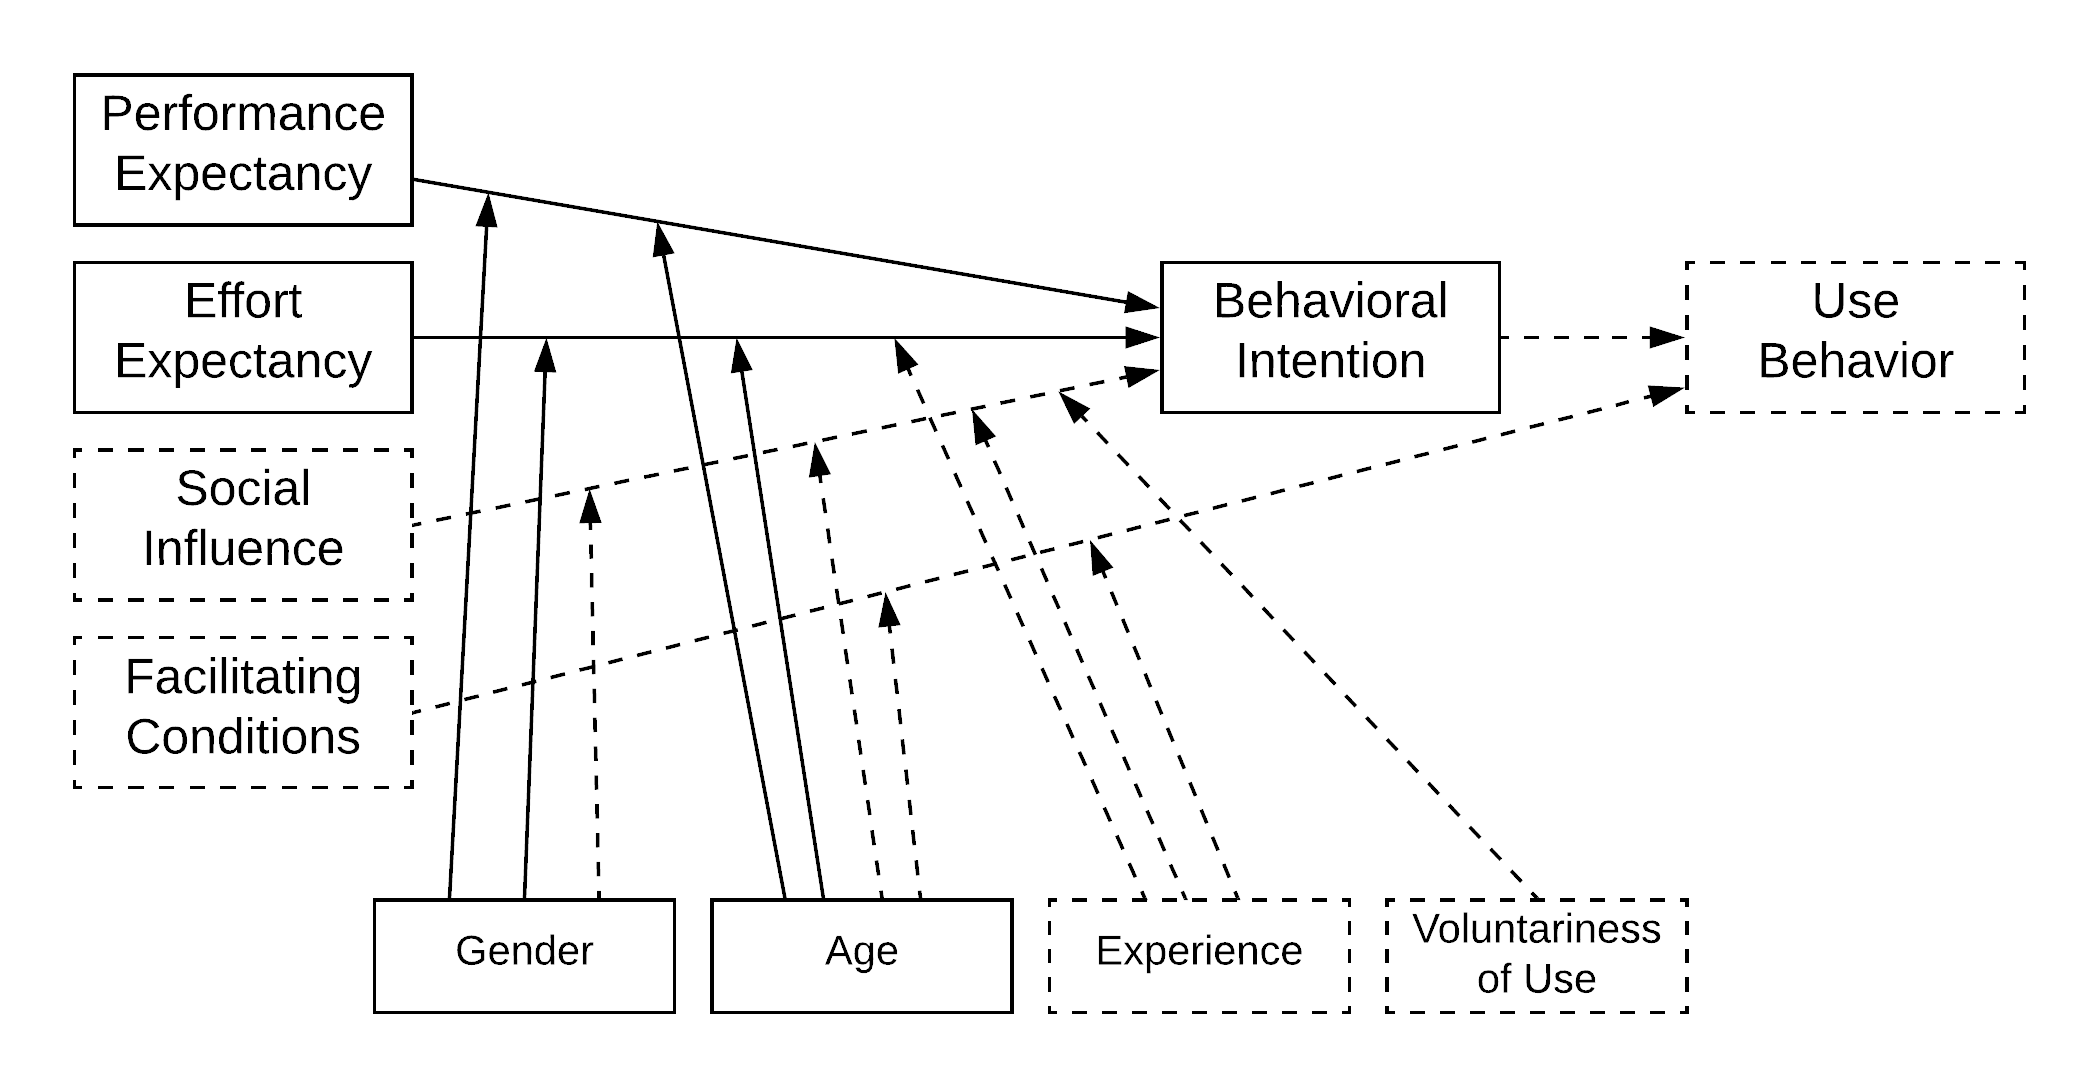
\includegraphics[scale=0.2]{figures/UTAUT.png}
    \caption{\acrshort{utaut} model \parencite[p. 447]{Venkatesh2003UserAO}}
    \label{fig:utaut}
\end{figure}

The current research paper applies the \acrshort{utaut} to examine how the different test groups evaluate \emph{Allergy Scan}. However, this analysis will be limited to the two most useful key factors for this application, namely performance expectancy and effort expectancy. Furthermore, the focus will be laid solely at the age and the gender of the participants (\cref{fig:utaut}).


\subsection{Performance Expectancy}
\textcite{Venkatesh2003UserAO} define performance expectancy as \enquote{the degree to which an individual believes that using the system will help him or her to attain gains in job performance} (p. 447). Performance expectancy is regarded as the strongest predictor for the intention to use and consists of five more underlying sub-constructs: perceived usefulness, extrinsic motivation, job-fit, relative advantage and outcome expectation (pp. 448-449).

In order to ensure a realistic scope for the current research, only three of the above-mentioned sub-constructs will be considered: the degree to which a user thinks the application would enhance his or her task performance (perceived usefulness), the effect on the enhancement of the user's task (job-fit) and the received perception of the application being better than the precursor solution (relative advantage) (p. 449).

The user's age and gender do have an impact on the relationship between performance expectancy and intention to use: men show a strong tendency to be task-oriented (p. 449) and, especially younger men, are more lead by extrinsic rewards (p. 450). This contributes to a more distinct influence of performance expectancy on intention to use (p. 450).

\subsection{Effort Expectancy}
Effort expectancy describes how the degree of ease of use of a particular technology \parencite[p. 450]{Venkatesh2003UserAO} has a significant impact on user acceptance and usage behavior (p. 447). Furthermore, this construct is composed of perceived ease of use (the perceived degree of being free of effort), complexity (the perception of being relatively difficult to understand to use) and ease of use (the perception of being difficult to use) (p. 451).

There is strong evidence that the user's age and gender have a significant impact: the effect of effort expectancy on intention to use is higher, particularly for younger women (p. 450).
